\begin{boxC}

    \begin{enumerate}
        \item 
        این زبان منظم متن را بر اساس 
        \textbf{کلمه}
        توکن توکن خواهد کرد.

        در زبان منظم 
        \lr{b}
        به عنوان مرز بین دو کاراکتر
        \lr{w (whitespace)}
        تعریف می‌شود.

        از این بابت مطمئن خواهیم بود که این جداکننده ، کلمات را بر اساس
        \textbf{کلمه}         
        جدا خواهد کرد ، نه بر اساس زیرکلمه و یا کاراکتر.

        همچنین با اجرای کد در بخش دوم از این بابت مطمئن خواهیم شد.
        
        \item 
        طبیعتا از اصلی‌ترین ایراداتی که در 
        \lr{tokenizer}
        بالا مشاهده می‌شود ، در درجه نخست ناتوانی در نمایش کامل 
        \textbf{تاریخ}
        و همچنین عدم نمایش کامل کلمه 
        \textbf{\lr{M.Sc.}}
        می‌باشد.

        یعنی 
        \lr{tokenizer}
        متوجه نشده‌است که این دو کلمه یک کلمه مستقل هستند و نباید 
        \lr{parse}
        شوند.

        این‌گونه می‌توان استدلال کرد که باید کاراکترهای 
        \lr{whitespace}
        را محدودتر نمود تا این زبان منظم هر کاراکتری را به عنوان
        \lr{whitespace}
        نپذیرد.

        \item 
        در زبان منظم اصلاح‌شده بعضی کاراکترهای معروف مثل 
        \textbf{آپاستروف}
        ،
        \textbf{\lr{dash}}
        ،
        \textbf{نقطه}
        و
        \textbf{\lr{backslash}}
        را به عنوان 
        \lr{whitespace}
        در نظرنگرفته‌ایم.

        در شکل ۲ می‌توانید کد آن را مشاهده بفرمایید.
    \end{enumerate}
    
\end{boxC}

% \includegraphics[width = \textwidth]
% {nlp1/images/q1-2.png}

\begin{figure}[h]
    \centering
    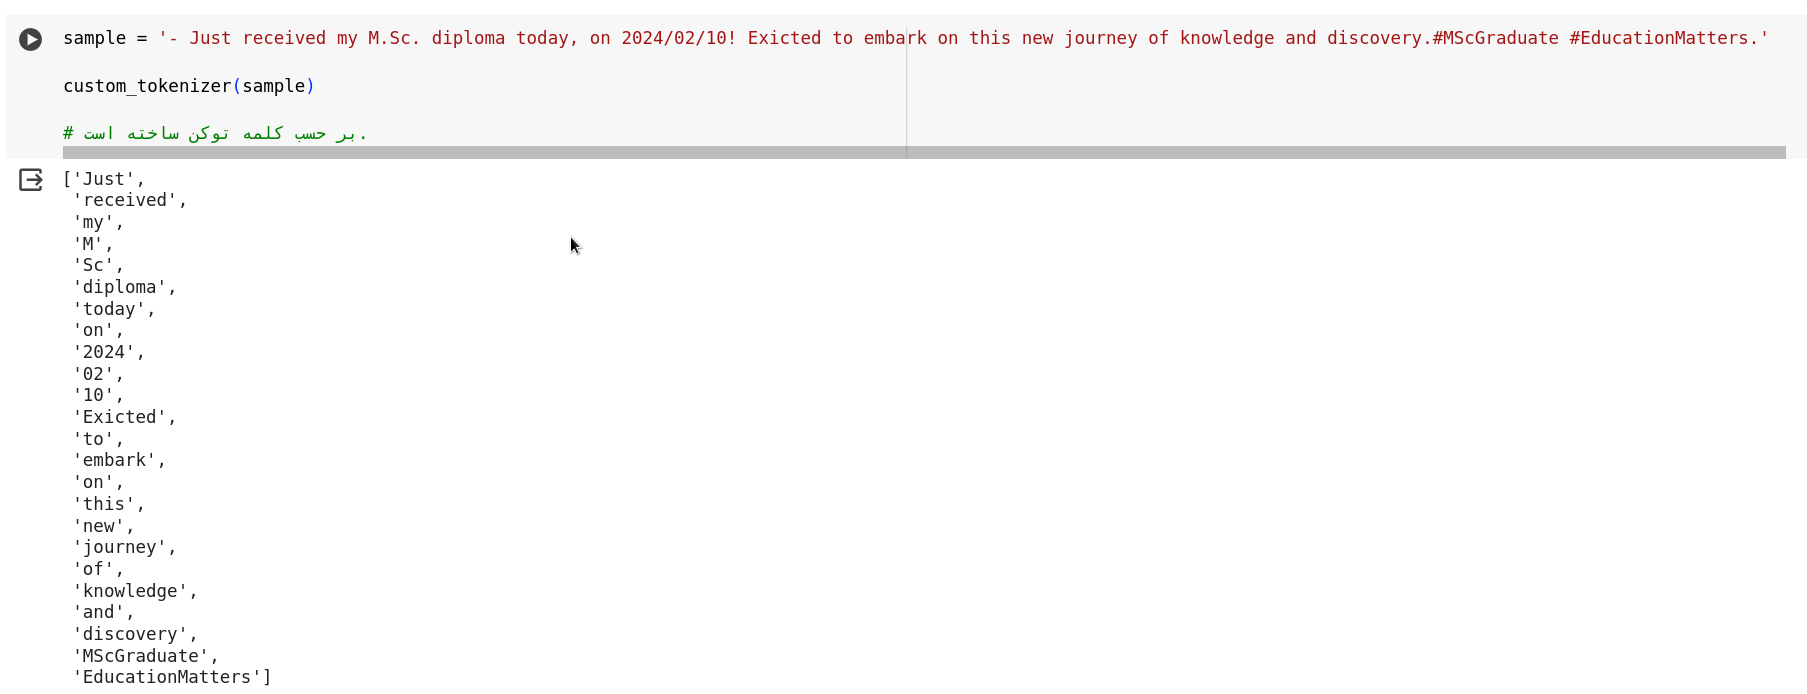
\includegraphics
    [width = 0.95\textwidth]
    {nlp1/images/q1-2.png}
    \caption{\lr{First Version of tokenizer and tokens}}
    \label{fig:enter-label}
\end{figure}


\begin{figure}[h]
    \centering
    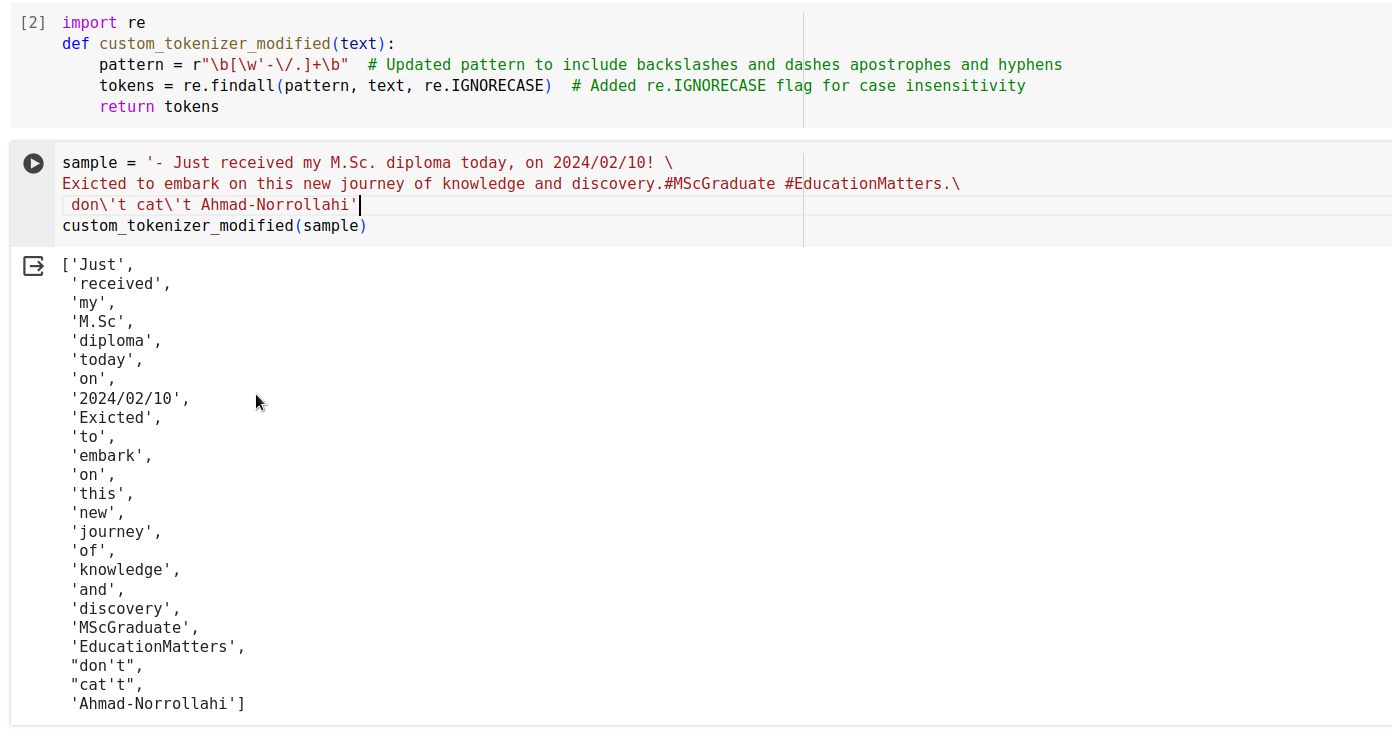
\includegraphics
    [width = 0.8\textwidth]
    {nlp1/images/q1-3.png}
    \caption{\lr{Modified Version of tokenizer and tokens}}
    \label{fig:enter-label}
\end{figure}


